%!TEX root=../tax-democracy-held.tex

\chapter{Common Grounds} \label{chap:common-grounds}

%here used to be \ref{fig:diss-mindmap}, but is now only in abstract

\begin{quote}
	\emph{``No man is an island, entire of itself every man is a piece of the continent, a part of the main if a clod be washed away by the sea, Europe is the less, as well as if a promontory were, as well as if a manor of thy friends or of thine own were any man’s death diminishes me, because I am involved in mankind and therefore never send to know for whom the bell tolls it tolls for thee.''}\\
	--- John Donne
\end{quote}

%the savings rate is, as I have explained an essentially political decision.


\begin{quote}
	\emph{``I am my brothers keeper. I am my sisters keeper.''}\\
	--- Barack Obama / Genesis 4, 9 KJV
\end{quote}


\section{Justice}

\subsection{The Evolution of Justice}

%--
%Compare two standards of justice and what they might do (both are pretty minimal actually). One is Rawlsian. The other is, as R. Frank has recently argued from a libertarian standpoint ``what-if-all-Coase-theorems'' could be resolved (with only the minimal empirical agreement on positional consumption, or as Frank puts it ``much of life is graded on the curve''. This is an interesting case. I don't know which one to do yet.

%I think I need some sort of substantive justice yardstick, otherwise what with the guy who says I just don't care about other people? What with the guy who says I want no taxes?  Just as deliberative democracy is an exercise in intersubjectivity, so must be the justice that underlies it. This is an axiomatic point, or maybe an anthropological one. Who we are as a species. Maybe Rawls justice as fairness will work here?

\section{Equality}

\begin{quote}
	\emph{``The hopes of the Republic cannot forever tolerate either undeserved poverty or self-serving wealth.''}\\*
	--- Franklin D. Roosevelt (Washington, DC, 1941)
\end{quote}

\begin{quote}
	\emph{``'Tis very certain that each man carries in his eye the exact indication of his rank in the immense scale of men, and we are always learning to read it.''}\\*
	--- Ralph Waldo \cite{Emerson1860}
\end{quote}

 \begin{figure}[htbp]
	\centering
	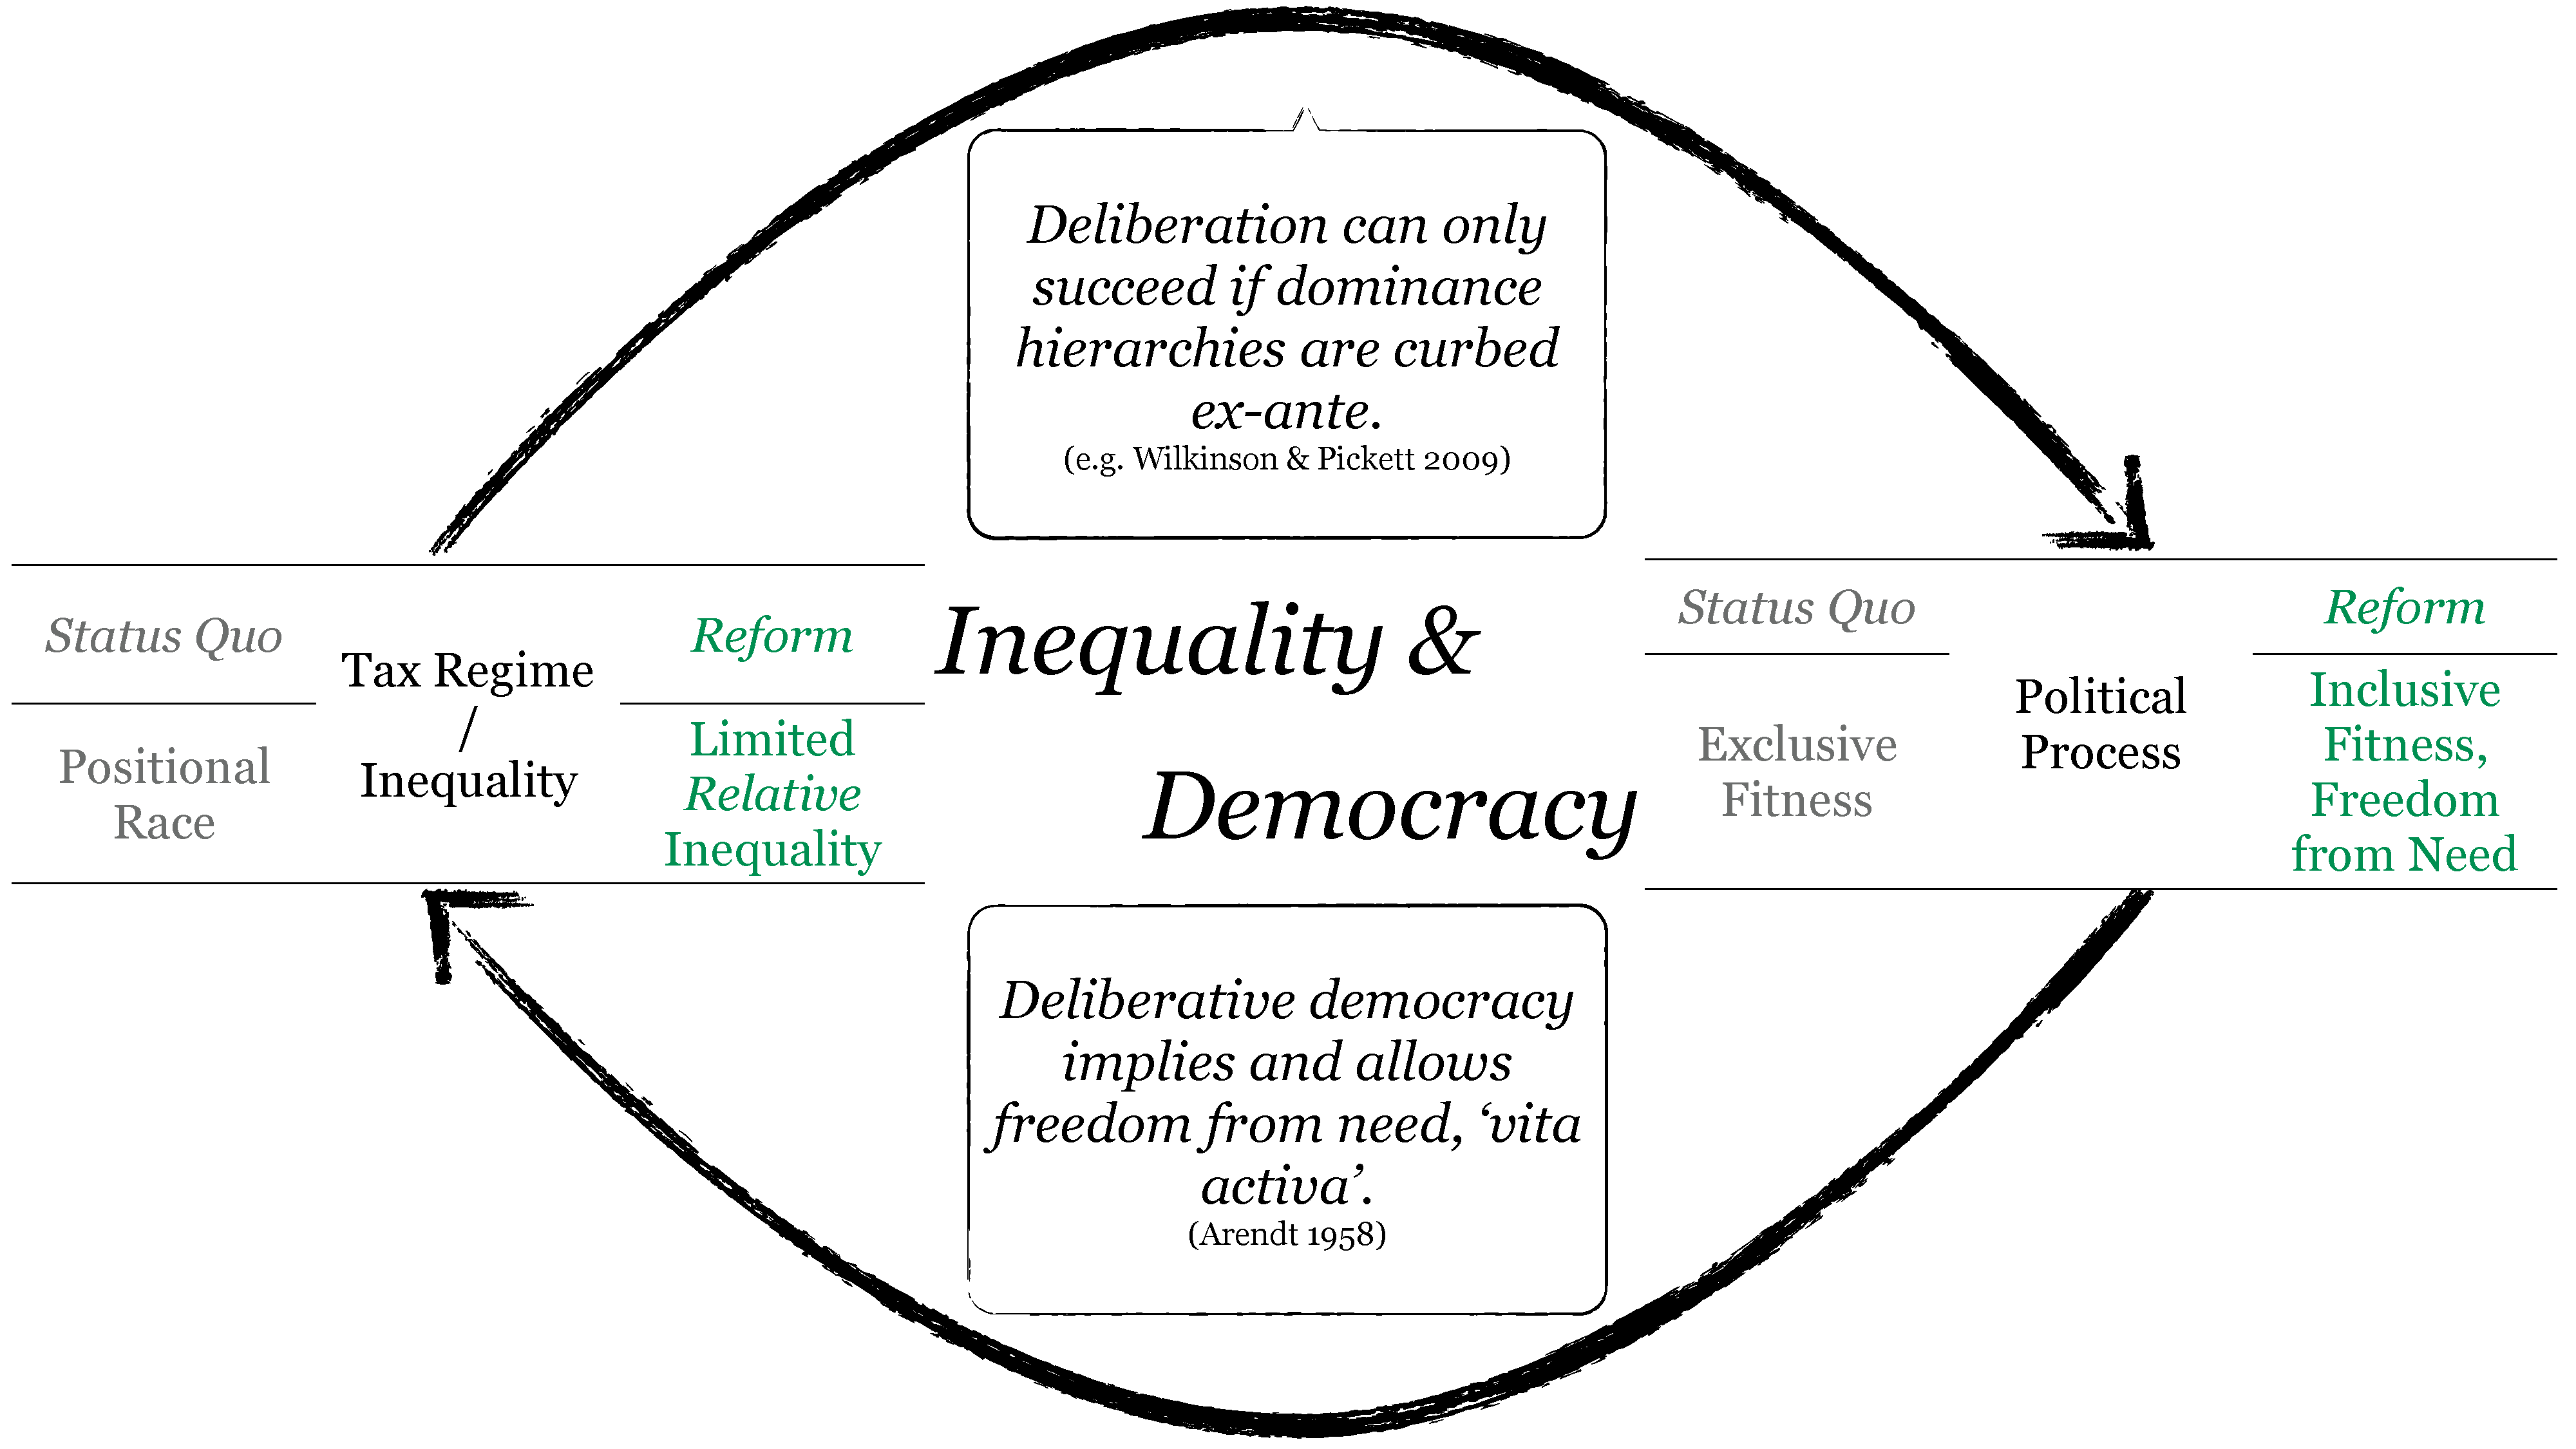
\includegraphics[width=1\linewidth]{inequality-democracy}
	\caption{Inequality and Democracy}
	\label{fig:inequality-democracy}
\end{figure}

%John Steinbeck: Socialism never took root in America because the poor see themselves not as an exploited proletariat, but as temporarily embarrassed millionaires


%key: "affiliative strategies are frequency dependent" (wright) -- which might suggest that deliberation does not work well under great inequality
	%this thing raises some questions whether I really believe in homo oec. Need to discuss this. I think it still works; affiliative strategies are, as Wright reminds us, frequency dependent, and may reside not just in genes, but in memes, too. And so it requires institutions to built on top of that. State and market are but ways to organize large-scale cooperation. At that, they're pretty good. We must not confuse the means by which they get us to do stuff (incentives) with the ends (inequality).
	%\cite{Wright1994}: reciprocal altruism evolved at the individual level, 	not at the group level (anything else would be falling for the group-selectionism bias). Tit for tat, as Axelrod has shown, is a winning strategy, but it is ``frequency dependent'' to be fit, meaning, you've got to encounter plenty of people with the same gene/meme. Reciprocal altruism is fairly rare in the animal kingdom. Wright speculates that recirprocal altruism (or tit for tat), which is vulnerable in to cheating in a crowd of non-cooperators might have gotten its initial boost from genetic nepotism (Hamilton). Both of these are strategies of inclusive fitness, because they also consider the addition inf itness to someone else. Also, note that reciprocal altruism is the kind of thing that you need if you're to become rich and functionally differentiated.
	%also look into this, via Wikipedia: According to Tim Dean, current scientific evidence confirms that humans do take diverse approaches to morality, and such polymorphism gives humanity resilience against a wider range of situations and environments (which makes moral diversity a natural consequence of frequency-dependent selection).[9] [10] [11] [12]

%First, despite literally hundreds of papers on the topic (Axelrod and D’Ambrosio 1994 lists 209 publications from 1987 to 1993), the theoretical conclusions derived for the mathematical models and computer simulations are substantially more ambiguous, nuanced, and qualified than those for kinship. Second, the empirical evidence for reciprocity-based cooperation in nonhuman species is scant (Hammerstein 2003), especially when compared to the evidence for kin-based cooperation. Nevertheless, in our species, reciprocity consistently emerges in both ethnographic and experimental studies.Read more at location 1064   • Delete this highlight
	%Note: reciprocity. note that this is the same word as gutman. also note reciprocity may be the one norm that isnt ambiguous as ethnicity nepotism et al. consider mirro neurons Edit

%schools as the operative metaphor for democracy
	%this is via the guy from UCI
	% and also from Dewey, via Wikipedia: "Dewey also criticized the dichotomy between means and ends which he saw as responsible for the degradation of our everyday working lives and education, both conceived as merely a means to an end. He stressed the need for meaningful labor and a conception of education that viewed it not as a preparation for life but as life itself. (Dewey 2004 [1910] ch. 7; Dewey 1997 [1938], p. 47)"

%Equal intrinsic worth!
%There's always the problem in democracy of equality

\subsection{The Evolution of Equality}

\section{Cooperation}

%Both pct (its political exonony of property, its idea of positional consumption, ita idea of taking stuff out of the communal cake) and deliberation (communication, it's idea of the human psyche) share an underlying theme: the social mind. We're much more relational thank we think.

%David Brooks: The social animal | Video on TED.com
	%"Over the past few years, we've been given a deeper view of human nature, and of who we are. (...). It's in the study of the mind: (...) we're developing a revolutionary consciousness. (...) It's giving us a new view of human nature, and far from being a coldly materialist human nature, it's a new humanism, a new enchantment.
	%(...) We're not primarily self-contained individuals. We're social animals, not rational animals. We emerge out of relationships, and we are deeply interpenetrated one with another."

%Deliberation needs trust.
%It appears that empirically (WP) and theoretically (WP, sociobiology of cooperation) that trust and inequality go together. Why? Inclusive fitness.

%Eichmann has no language and no recirpoviry and mutuality at all, he speaks in klishees. This Arendt (ch 2) says insulates him from everyone else.


%Deliberation is more than a method, here.
%Tax is more than a case, here.
%How Do We Get The Perfect Tax?

%Both pct (its political exonony of property, its idea of positional consumption, ita idea of taking stuff out of the communal cake) and deliberation (communication, it's idea of the human psyche) share an underlying theme: the social mind. We're much more relational thank we think.

 %Add Tax+democracy pic here
	%actually, that's already in "why hypotheticals matter"


%is there some argument to be made that INEQUALITY looms large in both tax, and deliberation?
	%**
	%Idea: there are two empirical, socio-biological questions that need to be reviewed: is there evidence for us being context-sensitive, graded on the curve? 2) what is the condition of our cooperation? How can we get us there?

%Wilkinson/Pickett
%"No mans is an Island, entire of itself; every man is a piece of the continent, a part of the main."
%(John Donne, MEditation XVII)

%Joseph und seine Brüder?

%is inequality what looms over both democracy and tax?
%Cohen and Rogers (1983: 157, as cited in Sanders) require ``the absence of material deprivation as a precondition for free and unconstrained deliberation'' and war that ``material inequalities can subvert a structure of free and equal public deliberation by translating into sharply unequal capacities for political action'' (ibid.: 158). Note how tax is a good case here: It's very challenging cognitively, but it's also very likely to invoke different SES standing, and, what's more, these two are likely to coincide. That sounds pretty bad, generally, but it's also good news for this research. Tax is, in fact, one of the hardest cases to possibly test deliberation.
	%again:cognition(Rosenberg)

%	\input{.tex/integration}


%there are questions that the PCT raises even if you share only very few political axioms.

% need to establish a convincing theoretical link between tax and deliberation

% The basic notion is that (democratic) process affects (democratic) outcome.


\subsection{Evolution of Cooperation}
%why sociobiology matters to this thesis
	%we have greater capacities (for reciprocal altruism) then is commonly assumed in late consumer capitalism
	%our capacity for reciprocal altruism depends on small locality and otherwise, on context. Today, tax is one of the institutions to build context for such altruism
	%status hurts us, badly. if we can do without status, we should. Apparently, there IS another resource to get us to do great things.
	%A deep if empuirically cursory understanding of evolved human nature will be important to figure out the ultimate needs that tax and deliberation will have to meet, and the conflicts both are likely to encounter.
	%deliberation is the ultimate, enlightened institution: no longer do we let self-interest build institutions (self-interest, collectively is an aimless process! It (capitalism, representative democracy) is an evolved institution!. Now we take things in our own hands.

%Need to look into the Kin and Kind article (brilliant) via The New Yorker in latest developments in inclusive fitness theory. http://www.newyorker.com/reporting/2012/03/05/120305fa-fact-lehrer

%random note, inspired by Wright, I think, from 10.07.2012
	%utilitarianism is the anti-thesis to evolution. In evolution, it's everyone for himself, and those are likely the values instilled in us by evolution. Notice that reciprocal altruism and nepotism are kind of stop-gap measures, by accident, almost, to get us to do a liittle bit of utilitarianism. These are tricks that evolution, and later, culture, played on this deficiency of humans, and all organisms to be endlessly self-seeking, or rather of genes being endlessely self-seeking. Here's a thought: utilitarianism fits uneasily with DIFFERENCE, it assumes that you can maximize the greatest good for the greatest many, that doesn't consider difference. Maybe deliberation is the synthesis: it puts everything up for grab, so it kind of shares the allocative norm of utilitarianism, but it allows for the possibiluty that people may define their own happinesses differently, and that we may not be able to consolidate all of this into one measure. We might want to do that, we don't know much about the ontology of difference, let alone the epistemology, but we accept it, not matter how it came about, even it may be false class consciousness. We accept difference, because we beleive in "autonomy" (dahl).
	%the other point is on utilitarianism, as the antithesis to evolution. Spread the greatest good for the greatest many, entirely equally. Which is the opposite to Pareto-optimisation, it's not what markets do, and not what evolution does. But WE as people escaped from the cosntraints of nature (autonomy, autarky), the cosntraints that all other animals lived under, by being the prime social beings. That's saying that we were equipped with a machinery to overcome our selfish impulses and cooperate. We are not necessarily smarter than chimps (cf. working memory), what we are is SOCIALLY smarter, and that is why (link this to arithmetric vs geometric growth): we escaped linear production functions, we got to economies of scale through cooperation. It's only a matter of consequence to continue down that road, if anything, that may be our destiny. This is a historical argument, if we got to the argument we are now, by cooperation, (cite Tilly, sociology of markets) to point out that at the bottom of the modern economy is an enormous ffeat of cooperation (tilly), without markets would never have come about. So if this is the history of the place we're in today, there's no reason to assume, it makes sense to apply the same logic and to further extent the limits of generosity and recirprocity, to further limit selfishness. This again, is an argument against a foundational notion: uncoerced exchange is legimiate (this applies to property, privile). The "uncoerced" part is wrong; this hyperliberal argument isn't true systematically and historically, because the very essence of surplus production (bingo) is cooperation. You cannot have surplus production without cooperation. So you should extent the realm of surplus production. This is the physical condition we live under. This is the physical condition we live under: non-zero sumness, it's everywhere from the PD to geometric growth.

%pluralist democracies, as markets, work on self-interest. They are fundamentally impoverished view os human nature, they don't follow this idea. Pluralist democracies are the extension of the market logic to the state. That doesn't work. Normatively, how it should be, is that markets are the place that governs the institutions, markets govern those tasks and only to the extent that we are unable to overcome our selfish demons. Only then, when we figure out we're not that good in producting smartphones without our selfish demons, than we allow for markets. we allow inequality. The other institution that doesn't allow for this is NOT the old (tillian) State, just a huge natural monopolist, but a deliberative polity is that institution that allows us to work on our unselfish demons, because we have those, too. We are somewhere in between. Our altruistic capacity in evolution wasn't built with any noble intention, it was just an accident, by which we were able to harvest economy of scale and to harvest non-zero-sumness. It grew, because non-zero-sumness was such a harbinger, because there was such wealth to be reaped. We insist on this today to remind us that we're lucky that we've got that altruistic capacity, too, by accident - but we've got it. And that's good news. So, pluralistic democracy is bad. And I'll show the dysfunctions, and these dysfunctions are one of two things. 1) they are how they hurt equality. and 2) how it hurts efficiency, because it doesn't account for non-zero-sumness that governs this realm of stuff that states are supposed to govern. In one sence, deliberation is a way to move the state from governing a homo economicus by force, to someplace else. I still have to think about this: i still want a strong state; in imeplementing it's policies it still relies on homo oec. This is how it might work: as we extent the reach and breadth of deliberation, this border shifts: the state relies less on violence, and more on understanding, on reciprocity.
	%small addition to Huxley, this is the progress of civilization, according to Wright. Peter Singer, "the more you know about your enemye, the more likely you are to win against it". That is the normative/political/ontological position of evolutionary psychology.

%work Arendt in here.

\section{Developmental Psychology}
%Rousseau: Emile
%Die Frage der Autonomie
%Rosenberg
%Lawrence Kohlberg
%Piaget?
%Freud?
%Liberale Theoriev
%Soziobiologie und spiegelneuronen

%Spiel Text von verena
%Entwicklungspsychologie ähnlich wie Rosenberg via Verena "Stufen der moralischen Entwicklung"
%Einführung in die entwicklungspsychologie etwa erikson
%Kasztantowicz, Ulrich über sonderschulpadagogil lesen: Verena sagt, das Thema ihrer Svhule ist Umgang mit Heterogenität.

%Gemeinwohl ist nicht für alle dasselbe, sagt Verena sagt Kohlberg.
%Was sagt John Rawls?
%Rousseau: contrat Social UND Emile

%Democracy and Education Form a Circle

%Pädagogik (Bildung) und demokratietheorie verhandeln beide Autonomie vs. Aufklärung/lernen/
%Sowie auch wuchtig sagt Verena ist lerntheorie (behaviorismus: Lob und Strafe, vs. Constructivism vs instruktionalismus

%---
%Ganz andere Idee für Verenas ba Arbeit: inklsuoln sind 3 Menschen vor Wand Treppe und Fahrstuhl auf dem weg zur ubahn. Fahrstuhl ist inklusive.
%Jetzt mal denken an 7. Klasse schlechter Migrationshintergrund Schuler der 3. Klasse hilft. Ist das nicht etwas anderes? Inklusion oder SOLiDARiTAt? Die Metapher hier ist: blinder und lahmer! (biblische konstante!). Wchselseitiges helfen es ist unklar wer wem hilft.
%Und was hat das alles mit deliberation zu tun?
%What if you can make deliberation into blinder und lahmer situations? What kind of trust do you need?
%Biographical information: I've never learnt as mich as when I was teaching.
%Autismus und Deliberation und Asperger.